\documentclass[12pt,a4paper]{article}
\usepackage[T1]{fontenc}
\usepackage[utf8]{inputenc}
\usepackage{mathptmx}
\renewcommand{\figurename}{Figura}
\renewcommand{\tablename}{Tabela}
\usepackage[a4paper,left=3cm,right=3cm,top=2.5cm,bottom=2.5cm]{geometry}
\usepackage{amsmath,amssymb,amsthm}
\usepackage{graphicx}
\usepackage{booktabs}
\usepackage{algorithm}
\usepackage{algpseudocode}
\usepackage{tikz}
\usepackage[square,authoryear]{natbib}
\usepackage[colorlinks=true,linkcolor=black,citecolor=black,urlcolor=black]{hyperref}
\usepackage{url}
\usepackage{caption}
\captionsetup{font=small,labelfont=bf,labelsep=period,justification=centering}
\usetikzlibrary{positioning,arrows.meta}

\setlength{\parindent}{1.0cm}
\setlength{\parskip}{0pt}
\renewcommand{\baselinestretch}{1.0}

% títulos de seção no estilo SBC (negrito, sem serifa especial)
\makeatletter
\renewcommand{\section}{\@startsection{section}{1}{0pt}{-14pt plus -2pt minus -1pt}{6pt}{\normalfont\large\bfseries}}
\renewcommand{\subsection}{\@startsection{subsection}{2}{0pt}{-10pt plus -2pt minus -1pt}{4pt}{\normalfont\normalsize\bfseries}}
\makeatother

% resumo e abstract no estilo SBC (itálico, recuado)
\newenvironment{resumobloco}[1]
  {\begin{list}{}{\setlength{\leftmargin}{0.8cm}\setlength{\rightmargin}{0.8cm}\setlength{\itemindent}{0pt}\setlength{\listparindent}{0pt}}
   \item[]\small\itshape\textbf{#1.}\ }
  {\end{list}}

\theoremstyle{plain}
\newtheorem{lema}{Lema}
\newtheorem{teorema}{Teorema}
\theoremstyle{definition}
\newtheorem*{prova}{Demonstração}

% citações no formato do Trabalho 1: [Autor et al. 2002]
\renewcommand{\cite}{\citep}
\bibpunct[, ]{[}{]}{;}{a}{}{,}
\algrenewcommand\algorithmicrequire{\textbf{Entrada:}}
\algrenewcommand\algorithmicensure{\textbf{Saída:}}
\algrenewcommand\algorithmicif{\textbf{se}}
\algrenewcommand\algorithmicthen{\textbf{então}}
\algrenewcommand\algorithmicfor{\textbf{para}}
\algrenewcommand\algorithmicdo{\textbf{faça}}
\algrenewcommand\algorithmicreturn{\textbf{devolva}}
\algrenewcommand\algorithmicwhile{\textbf{enquanto}}
\algrenewcommand\algorithmicelse{\textbf{senão}}
\algrenewcommand\algorithmicend{\textbf{fim}}
\algrenewcommand\algorithmicforall{\textbf{para todo}}
\algrenewtext{EndIf}{\algorithmicend\ \algorithmicif}
\algrenewtext{EndFor}{\algorithmicend\ \algorithmicfor}
\algrenewtext{EndWhile}{\algorithmicend\ \algorithmicwhile}
\algrenewtext{EndProcedure}{\algorithmicend\ \algorithmicprocedure}
\renewcommand{\algorithmicprocedure}{\textbf{procedimento}}
\floatname{algorithm}{Algoritmo}

\begin{document}
\begin{center}
{\Large\bfseries Corte Máximo: Algoritmos Exatos por Branch-and-Bound\\ e Programação Dinâmica sobre a Largura de Caminho}\\[10pt]
{\bfseries Eduardo Marinho$^1$, Marcos Fontes$^1$}\\[6pt]
$^1$Centro de Ciências Exatas e da Terra\\
Departamento de Informática e Matemática Aplicada (DIMAp)\\
Universidade Federal do Rio Grande do Norte (UFRN) -- Natal, RN -- Brasil\\
DIM0605 -- Projeto e Análise de Algoritmos -- Prof.\ Sílvia Maia\\
Novembro de 2026
\end{center}
\vspace{6pt}
\begin{resumobloco}{Abstract}
This paper presents two exact algorithms for the Maximum Cut problem: a Branch-and-Bound with an incrementally maintained upper bound, initialized with the greedy local-search heuristic of our previous work, and a dynamic program over the frontier of a vertex ordering, whose cost is exponential only in the pathwidth of the ordering. Both are proved correct and were validated against brute force on 3,000 small random graphs. On 79 instances, the dynamic program solved every sparse random graph up to 120 vertices and toroidal grids with $\pm1$ weights of up to 2,000 vertices in about 12 s or less, while Branch-and-Bound solved random graphs up to about 80 vertices and could not prove optimality on any grid. With the optima at hand, the previous heuristic reaches 77--80\% of the optimum on the 2,000-vertex toroidal grids and 91--98\% on sparse random graphs with positive weights.
\end{resumobloco}
\vspace{8pt}
\begin{resumobloco}{Resumo}
Este trabalho apresenta dois algoritmos exatos para o problema do Corte Máximo: um Branch-and-Bound com limitante superior mantido de forma incremental e inicializado com a heurística gulosa com busca local do trabalho anterior, e uma programação dinâmica sobre a fronteira de uma ordem dos vértices, cujo custo é exponencial apenas na largura de caminho da ordem. Ambos têm prova de correção e foram validados contra força bruta em 3\,000 grafos aleatórios pequenos. Em 79 instâncias, a programação dinâmica resolveu todos os grafos aleatórios esparsos até 120 vértices e grades toroidais com pesos $\pm1$ de até 2\,000 vértices em até cerca de 12\,s, enquanto o Branch-and-Bound resolveu grafos aleatórios até cerca de 80 vértices e não provou a otimalidade de nenhuma grade. Com os ótimos em mãos, a heurística do trabalho anterior obtém de 77 a 80\% do ótimo nas grades toroidais de 2\,000 vértices e de 91 a 98\% em grafos aleatórios esparsos com pesos positivos.
\end{resumobloco}
\section{Introdução}

O problema do Corte Máximo (\emph{Max-Cut}) consiste em dividir os vértices de um grafo em dois grupos de modo que o peso total das arestas entre os grupos seja o maior possível. No Trabalho~1 estudamos uma heurística gulosa com busca local 1-flip, que processa grafos de 100 mil vértices em milissegundos, mas não dá nenhuma garantia além de $1/2$ do ótimo e, nos grafos toroidais com pesos $\pm1$ do G-set, ficou em torno de 80\% do melhor valor conhecido. Esse número, porém, é relativo a valores obtidos por metaheurísticas \cite{Benlic and Hao 2013}, e não ao ótimo: não sabíamos o quanto da diferença era culpa da heurística e o quanto vinha de uma referência que também pode estar abaixo do ótimo.

Este trabalho aborda a outra ponta do problema: algoritmos \emph{exatos}, que sempre devolvem o ótimo e provam que ele é o ótimo, ao custo de tempo exponencial no pior caso. Implementamos dois, de técnicas diferentes. O primeiro é um \emph{Branch-and-Bound} com um limitante superior atualizado de forma incremental e inicializado com a heurística do Trabalho~1. O segundo é uma \emph{programação dinâmica sobre a largura de caminho} do grafo, que explora o fato de os grafos esparsos poderem ser processados com uma ``fronteira'' pequena de vértices ativos. Os dois foram validados contra força bruta em 3\,000 grafos aleatórios pequenos e comparados entre si e com a heurística do Trabalho~1 em 79 instâncias.

Um resultado negativo precisa ser dito logo: nenhum algoritmo exato escrito do zero resolve as instâncias do G-set usadas no Trabalho~1 (2\,000 a 20\,000 vértices), e a literatura que resolve esses tamanhos recorre a ferramentas muito mais sofisticadas \cite{Liers et al. 2004, Rendl et al. 2010}. Por isso as instâncias deste trabalho são menores ou têm estrutura favorável: grafos aleatórios esparsos de 20 a 120 vértices, com o mesmo gerador do Trabalho~1, e grades toroidais $\pm1$ de até 2\,000 vértices, o mesmo porte do G32, mas com largura pequena. A Seção~\ref{sec:instancias} justifica a escolha.

O artigo segue a ordem pedida: as Seções~2 e~3 descrevem o problema, sua complexidade e o estado da arte em algoritmos exatos; a Seção~4 justifica as duas técnicas; a Seção~5 apresenta os algoritmos com provas de correção e análise de complexidade; a Seção~6 descreve as instâncias e a metodologia de teste; a Seção~7 traz os resultados e a comparação com o Trabalho~1; a Seção~8 conclui.

\section{Descrição do Problema e Complexidade}

Seja $G=(V,E)$ um grafo não direcionado com $n=|V|$ vértices e $m=|E|$ arestas, em que cada aresta $uv$ tem um peso inteiro $w_{uv}$. Uma partição é uma função $s:V\to\{0,1\}$, e o valor do corte é
\begin{equation}
  \mathrm{cut}(s)=\sum_{uv\in E,\; s(u)\neq s(v)} w_{uv}.
\end{equation}
O problema pede uma partição de valor máximo, $\mathrm{OPT}=\max_s \mathrm{cut}(s)$. Usamos a mesma notação do Trabalho~1: $N(v)$ é a vizinhança de $v$, $\Delta$ é o grau máximo e $W=\sum_{uv\in E}|w_{uv}|$.

\subsection{Complexidade}

A versão de decisão (existe um corte de valor pelo menos $k$?) está em NP, pois uma partição é verificada em $O(n+m)$, e é NP-completa \cite{Karp 1972, Garey et al. 1976}. Logo a versão de otimização é NP-difícil e não se espera um algoritmo polinomial exato, a menos que P $=$ NP. Todo algoritmo exato conhecido para o caso geral leva tempo exponencial. A enumeração das $2^{n-1}$ partições (a menos de simetria) resolve o problema em tempo $O(2^n)$ com código de Gray, e o melhor limite de pior caso que conhecemos é o de \citet{Williams 2005}, de ordem $O(2^{\omega n/3})$ ($\omega$ é o expoente da multiplicação de matrizes), cerca de $1{,}73^n$, mas ao custo de memória também exponencial e sem utilidade prática em grafos esparsos.

Há casos tratáveis. Em grafos planares o problema é polinomial \cite{Hadlock 1975}, o que inclui as grades com contorno periódico em no máximo uma direção \cite{Liers et al. 2003}; o toro, periódico nas duas direções, que é a classe das nossas grades, não é planar. Em grafos de largura de caminho (ou de árvore) $w$, programação dinâmica resolve o problema em tempo $O(2^{w}\cdot \mathrm{poly}(n))$ \cite{Arnborg et al. 1991, Bodlaender 1993}, o que é a base do segundo algoritmo deste trabalho. Os dois extremos explicam a escolha de instâncias: o problema é tratável quando o grafo tem estrutura (largura pequena) e difícil quando não tem (grafos aleatórios), embora esparsos.

\section{Estado da Arte em Algoritmos Exatos}

Os métodos exatos práticos para o Max-Cut dividem-se em três famílias.

\paragraph{Branch-and-cut poliédrico.} Formulam o problema como programação linear sobre o politopo de corte e acrescentam desigualdades válidas (de ciclo ímpar, de triângulo, entre outras) durante a busca. \citet{Barahona et al. 1988} aplicaram essa abordagem a estados fundamentais de vidros de spin e ao projeto de circuitos, e \citet{Liers et al. 2004} descrevem o seu uso para vidros de spin difíceis. \citet{Liers et al. 2003} calcularam os estados fundamentais de vidros de spin em grafos aleatórios regulares de grau 4 e 6 (acoplamentos gaussianos) com até 1\,280 spins, uma classe próxima dos nossos grafos aleatórios esparsos ($m=2n$ tem grau médio 4), e observaram que o tempo cresce de forma polinomial na fase ferromagnética e mais que polinomial na fase de vidro de spin. Métodos poliédricos são, em geral, os mais indicados para grafos esparsos.

\paragraph{Branch-and-bound semidefinido.} Calculam os limitantes com a relaxação semidefinida do problema reforçada por desigualdades de triângulo. O \emph{Biq Mac} \cite{Rendl et al. 2010} resolve em tempo razoável qualquer instância de até $n=100$ vértices, qualquer que seja a densidade, e é o método de referência para grafos densos; os próprios autores observam que, para grafos esparsos, métodos baseados em programação linear podem ser preferíveis. \citet{Krislock et al. 2014} melhoraram o cálculo dos limitantes e relatam desempenho superior ao do Biq Mac na maior parte das instâncias testadas.

\paragraph{Exploração de estrutura.} Para grafos de largura de caminho ou de árvore pequena, a programação dinâmica sobre a decomposição é exata e de custo $O(2^{w}\mathrm{poly}(n))$ \cite{Arnborg et al. 1991, Bodlaender 1993}. A largura de caminho é igual ao número de separação de vértices de um melhor ordenamento \cite{Kinnersley 1992}, o que permite implementá-la como um percurso por uma ordem de vértices, como fazemos na Seção~5.2.

Nossos dois algoritmos ocupam posições modestas nesse panorama. O Branch-and-Bound usa um limitante barato, calculado em $O(\deg v)$ por nó, em vez de relaxações lineares ou semidefinidas; ele troca qualidade do limitante por velocidade por nó. A programação dinâmica é a versão mais simples da terceira família. Não esperamos competir com \emph{Biq Mac} ou com os resolvedores de branch-and-cut, e a comparação com a literatura da Seção~7 deve ser lida com esse cuidado.

\section{Técnicas Escolhidas}

\paragraph{Branch-and-Bound.} Constrói a partição vértice a vértice, ramificando nos dois lados possíveis, e poda um ramo quando um limitante superior do valor de qualquer completação não supera o melhor corte já conhecido. Não exige nenhuma estrutura do grafo e funciona com pesos de qualquer sinal; sua eficiência depende só da qualidade do limitante e da ordem de decisão. Usamos como limite inferior inicial a heurística do Trabalho~1, o que liga os dois trabalhos: uma heurística boa poda mais desde o primeiro nó.

\paragraph{Programação dinâmica sobre a fronteira.} Processa os vértices em uma ordem fixa e mantém, para cada atribuição possível dos vértices da \emph{fronteira} (processados que ainda têm vizinhos por processar), o melhor valor parcial. Quando um vértice perde o último vizinho pendente, ele sai da fronteira e o algoritmo maximiza sobre o seu lado. A Figura~\ref{fig:fronteira} ilustra o percurso. O custo é exponencial apenas na largura da fronteira, e não em $n$.

As duas técnicas são complementares. O Branch-and-Bound é geral, mas seu tempo explode com $n$ mesmo em grafos esparsos. A programação dinâmica depende da estrutura, mas, quando ela existe, resolve instâncias com milhares de vértices. Como o tema do Trabalho~1 foi grafos grandes e esparsos, a segunda técnica é a mais natural para o contraste com a heurística.

\begin{figure}[ht]
\centering
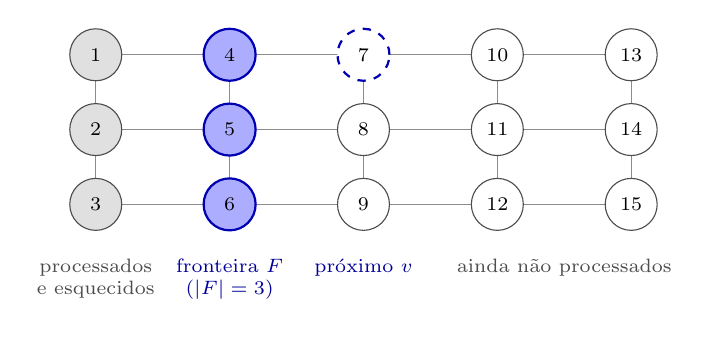
\begin{tikzpicture}[x=1.7cm,y=-0.95cm,
  vtx/.style={circle,draw=black!70,minimum size=0.66cm,inner sep=0pt,font=\scriptsize},
  proc/.style={vtx,fill=black!12},
  fron/.style={vtx,fill=blue!32,draw=blue!70!black,thick},
  prox/.style={vtx,fill=white,draw=blue!70!black,thick,dashed},
  nao/.style={vtx,fill=white},
  aresta/.style={draw=black!45}]
  \foreach \c in {1,...,5}{\foreach \r in {1,2,3}{
    \pgfmathtruncatemacro{\id}{(\c-1)*3+\r}
    \coordinate (p\c\r) at (\c,\r);
  }}
  \foreach \c in {1,...,5}{\foreach \r in {1,2,3}{
    \pgfmathtruncatemacro{\cc}{\c+1}\pgfmathtruncatemacro{\rr}{\r+1}
    \ifnum\c<5 \draw[aresta] (p\c\r) -- (p\cc\r); \fi
    \ifnum\r<3 \draw[aresta] (p\c\r) -- (p\c\rr); \fi
  }}
  \foreach \c/\sty in {1/proc,2/fron,3/nao,4/nao,5/nao}{\foreach \r in {1,2,3}{
    \pgfmathtruncatemacro{\id}{(\c-1)*3+\r}
    \ifnum\c=3\ifnum\r=1 \node[prox] at (p\c\r) {\id}; \else \node[nao] at (p\c\r) {\id}; \fi
    \else \node[\sty] at (p\c\r) {\id}; \fi
  }}
  \node[anchor=north,align=center,font=\scriptsize,text=black!70] at (1,3.6) {processados\\e esquecidos};
  \node[anchor=north,align=center,font=\scriptsize,text=blue!60!black] at (2,3.6) {fronteira $F$\\($|F|=3$)};
  \node[anchor=north,align=center,font=\scriptsize,text=blue!60!black] at (3,3.6) {próximo $v$};
  \node[anchor=north,align=center,font=\scriptsize,text=black!70] at (4.5,3.6) {ainda não processados};
\end{tikzpicture}
\caption{Percurso da programação dinâmica em uma grade $3\times5$ numerada por colunas. Os vértices 1 a 3 já saíram da fronteira (todos os seus vizinhos foram processados); os vértices 4 a 6 formam a fronteira $F$, porque cada um ainda tem vizinho na coluna seguinte. Ao inserir o vértice 7, a tabela tem $2^{|F|+1}=16$ entradas.}\label{fig:fronteira}
\end{figure}

\section{Algoritmos Implementados}

\subsection{Algoritmo 1: Branch-and-Bound}

Os vértices são decididos em uma ordem $\pi$ calculada de forma gulosa: começa-se pelo vértice de maior peso ponderado $\sum|w|$, e o próximo é sempre o que tem maior peso $|w|$ total para os já ordenados. Assim as arestas ficam ``decididas'' (as duas pontas fixadas) o mais cedo possível e o limitante se torna justo cedo. Quando o próximo vértice não tem nenhum vizinho já ordenado, ele abre uma nova componente conexa.

Em um nó da busca, os vértices $\pi_1,\dots,\pi_{i}$ estão decididos. Para cada vértice $v$ ainda não decidido mantemos $c_0(v)$ e $c_1(v)$, os pesos das arestas de $v$ para vizinhos já decididos nos lados 0 e 1. Colocar $v$ no lado $s$ corta exatamente as arestas para decididos do lado oposto, com ganho $c_{1-s}(v)$. Seja $\mathrm{cut}_\sigma$ o valor das arestas já decididas que estão cortadas. O limitante superior é
\begin{equation}\label{eq:ub}
  \mathrm{UB}(\sigma)=\mathrm{cut}_\sigma+\sum_{v\ \text{livre}}\max\{c_0(v),c_1(v)\}+\sum_{\substack{uv\in E\\ u,v\ \text{livres}}}\max\{w_{uv},0\}.
\end{equation}

\begin{lema}\label{lema:ub}
Para toda completação $s$ da solução parcial $\sigma$, $\mathrm{cut}(s)\le \mathrm{UB}(\sigma)$.
\end{lema}
\begin{prova}
Separe as arestas em três classes. As que têm as duas pontas decididas contribuem exatamente $\mathrm{cut}_\sigma$, qualquer que seja a completação. Uma aresta $uv$ com $v$ livre e $u$ decidido só é cortada se $v$ ficar do lado oposto de $u$; assim, o que as arestas de $v$ para decididos contribuem é $c_{1-s(v)}(v)\le\max\{c_0(v),c_1(v)\}$. Por fim, uma aresta entre dois livres contribui $w_{uv}$ ou $0$, no máximo $\max\{w_{uv},0\}$. Somando as três classes, obtém-se (\ref{eq:ub}). \qed
\end{prova}

As três parcelas de (\ref{eq:ub}) são mantidas de forma incremental: ao fixar $v$ no lado $s$, só mudam as parcelas de $v$ e de seus vizinhos livres, em tempo $O(\deg v)$, e o desfazer é simétrico. O algoritmo ramifica primeiro no lado que corta mais peso (o de maior ganho), pois isso tende a encontrar boas soluções cedo. Como o valor de uma partição não muda ao trocar os dois lados de uma componente inteira, o primeiro vértice de cada componente é fixado no lado 0, o que corta a busca pela metade por componente. O Algoritmo~\ref{alg:bb} resume o procedimento.

\begin{algorithm}[ht]
\caption{Branch-and-Bound}\label{alg:bb}
\begin{algorithmic}[1]
\Require grafo $G=(V,E,w)$, tempo máximo $T$
\Ensure partição $s^*$ de valor máximo (ou a melhor encontrada, se o tempo acabar)
\State $s^*\gets$ heurística do Trabalho 1; \quad $\mathit{melhor}\gets \mathrm{cut}(s^*)$
\State calcular a ordem $\pi$ e inicializar $c_0,c_1,\mathrm{cut}_\sigma,\mathrm{UB}$
\Procedure{Rec}{$i$}
  \If{$\mathrm{UB}(\sigma)\le \mathit{melhor}$} \State \textbf{retornar} \Comment{poda}
  \EndIf
  \If{$i=n$} \State $\mathit{melhor}\gets \mathrm{cut}_\sigma$; \quad $s^*\gets\sigma$; \quad \textbf{retornar}
  \EndIf
  \State $v\gets\pi_i$
  \For{$s\in\{0,1\}$, começando pelo lado de maior ganho \textbf{e pulando} $s=1$ se $v$ abre componente}
    \State fixar $v$ no lado $s$; \quad \Call{Rec}{$i+1$}; \quad desfazer
  \EndFor
\EndProcedure
\State \Call{Rec}{$0$}; \quad \textbf{devolva} $s^*$
\end{algorithmic}
\end{algorithm}

\begin{teorema}[Correção]\label{teo:bb}
Se o Algoritmo~\ref{alg:bb} termina sem estourar o tempo, $\mathrm{cut}(s^*)=\mathrm{OPT}$.
\end{teorema}
\begin{prova}
O valor $\mathit{melhor}$ é sempre o corte de uma partição válida ($s^*$), pois começa com a da heurística e só é atualizado em folhas, onde $\mathrm{UB}=\mathrm{cut}$. Suponha, por contradição, que exista $s'$ com $\mathrm{cut}(s')>\mathit{melhor}$ ao final. Pela simetria por componente, podemos supor que $s'$ tem lado 0 no primeiro vértice de cada componente, pois trocar todos os lados de uma componente preserva o valor do corte e não cria nem remove arestas cortadas entre componentes (não há arestas entre elas). Então $s'$ é uma folha da árvore completa de decisões. Em todo nó $\sigma$ do caminho até $s'$, o Lema~\ref{lema:ub} dá $\mathrm{UB}(\sigma)\ge\mathrm{cut}(s')>\mathit{melhor}_{\text{final}}$, e como $\mathit{melhor}$ só cresce, $\mathrm{UB}(\sigma)>\mathit{melhor}$ no momento da visita. Logo nenhum nó do caminho é podado, a folha $s'$ é visitada, e nela $\mathrm{cut}(s')>\mathit{melhor}$ faz o algoritmo atualizar $\mathit{melhor}$ para pelo menos $\mathrm{cut}(s')$, o que contradiz $\mathit{melhor}_{\text{final}}<\mathrm{cut}(s')$. \qed
\end{prova}

\paragraph{Complexidade.} Cada nó custa $O(\deg v)$, e a árvore tem no máximo $2^{n-c+1}$ nós ($c$ componentes), então o pior caso é $O(2^{n}\,\Delta)$ em tempo e $O(n+m)$ em memória. Não há garantia melhor: o limitante \eqref{eq:ub} é fraco quando a maior parte do peso fica em arestas entre vértices livres, de modo que o número de nós visitados cresce exponencialmente com $n$ na prática também, como mostra a Seção~7.

\subsection{Algoritmo 2: Programação dinâmica sobre a fronteira}

Dada uma ordem $\pi=(v_1,\dots,v_n)$, seja $P_i=\{v_1,\dots,v_i\}$ o conjunto dos $i$ primeiros vértices e
\[F_i=\{u\in P_i : u \text{ tem algum vizinho fora de } P_i\}\]
a \emph{fronteira}. Para $x\in\{0,1\}^{F_i}$, defina
\begin{equation}
  f_i(x)=\max\Big\{\sum_{\substack{uv\in E,\ u,v\in P_i\\ y_u\ne y_v}} w_{uv}\ :\ y\in\{0,1\}^{P_i},\ y|_{F_i}=x\Big\},
\end{equation}
o melhor valor, entre as arestas já completamente processadas, de uma atribuição que concorda com $x$ na fronteira. Temos $F_0=\emptyset$ e $f_0(\emptyset)=0$. O passo $i$ tem duas fases.

\emph{Inserção.} Os vizinhos de $v_i$ em $P_{i-1}$ pertencem todos a $F_{i-1}$, pois cada um tem $v_i$ como vizinho ainda não processado. Logo o ganho de colocar $v_i$ no lado $s$ depende só de $x$:
\begin{equation}
  h(x,s)=f_{i-1}(x)+\sum_{u\in N(v_i)\cap F_{i-1},\ x_u\ne s} w_{uv_i},\qquad x\in\{0,1\}^{F_{i-1}},\ s\in\{0,1\}.
\end{equation}
Se a fronteira está vazia, $v_i$ abre uma componente nova e fixamos $s=0$ (simetria). A tabela passa a ter $2^{|F_{i-1}|+1}$ entradas.

\emph{Esquecimento.} Todo $u$ na tabela que não tem mais vizinhos fora de $P_i$ é eliminado, por maximização sobre o seu lado: $f(x_{-u})=\max_{b\in\{0,1\}} h(x_{-u},x_u{=}b)$. O algoritmo guarda um bit por estado dizendo qual $b$ venceu. Ao final, $F_n=\emptyset$ e $f_n(\emptyset)=\mathrm{OPT}$. A partição ótima é recuperada percorrendo os passos em ordem inversa: em cada esquecimento, o bit guardado dá o lado do vértice eliminado.

\begin{teorema}[Correção]\label{teo:dp}
Para toda ordem $\pi$, a tabela $f_n$ calculada pelo algoritmo satisfaz $f_n(\emptyset)=\mathrm{OPT}$, e a partição reconstruída tem corte $\mathrm{OPT}$.
\end{teorema}
\begin{prova}
Por indução em $i$, mostramos que a tabela calculada coincide com $f_i$. A base é trivial. No passo de inserção, uma atribuição $y$ de $P_i$ é a de $P_{i-1}$ mais o lado $s$ de $v_i$; as arestas novas são as que ligam $v_i$ a $P_{i-1}$, todas com a outra ponta em $F_{i-1}$, e o seu valor depende só de $y|_{F_{i-1}}=x$ e de $s$, o que dá $h$. Maximizar sobre as atribuições de $P_{i-1}$ compatíveis com $x$ resulta em $f_{i-1}(x)+\text{ganho}(x,s)$. No esquecimento, um vértice $u$ eliminado não tem mais arestas para vértices não processados, então nenhuma aresta futura depende de $y_u$, e a maximização sobre $y_u$ não perde nenhuma completação. Para $i=n$ a fronteira é vazia e $f_n(\emptyset)$ é o máximo sobre todas as atribuições, que é $\mathrm{OPT}$. A restrição $s=0$ ao abrir componente não perde o ótimo, pelo mesmo argumento de simetria do Teorema~\ref{teo:bb}. A reconstrução desfaz as maximizações na ordem inversa, e o bit guardado em cada estado é o que realizou o máximo, logo a partição obtida atinge $f_n(\emptyset)$. \qed
\end{prova}

\paragraph{Complexidade.} Seja $w=\max_i(|F_{i-1}|+1)$, o tamanho em bits da maior tabela. A inserção do vértice $v_i$ percorre $2^{|F_{i-1}|}$ estados, cada um em $O(\deg^-(v_i))$ (vizinhos já processados); cada esquecimento custa $O(2^{w-1})$ e há $n$ no total. O tempo é $O(n\,2^{w}+2^{w}\,m)=O(2^{w}(n+m))$, e a memória, $O(2^{w})$ para duas tabelas mais $O(n\,2^{w})$ \emph{bits} para os ponteiros de reconstrução. O valor $w-1$ é o número de separação de vértices da ordem, e o mínimo sobre todas as ordens é a largura de caminho do grafo \cite{Kinnersley 1992}; portanto, com a melhor ordem, o tempo é $O(2^{\mathrm{pw}(G)+1}(n+m))$. Achar a melhor ordem é difícil; usamos a heurística descrita a seguir.

\paragraph{Escolha da ordem.} Um guloso que, a cada passo, escolhe entre os vértices adjacentes à fronteira aquele que minimiza o tamanho da fronteira resultante (desempate pelo menor número de vizinhos pendentes e, depois, ao acaso). A construção é repetida a partir de até 30 vértices iniciais diferentes (o primeiro, de menor grau) e fica-se com a ordem de menor $w$. Antes de alocar qualquer tabela, o programa simula a ordem para conhecer $w$ e a memória necessária e recusa a execução se $w>26$ (parâmetro) ou se a memória passar de 2\,GB. A Figura~\ref{fig:fronteira} mostra uma ordem que varre a grade pelo lado longo; é o que o guloso aparenta encontrar nas grades toroidais (fronteira de $2L$ vértices mais o vértice inserido, ou seja, $w=2L+1$, como se vê na Tabela~\ref{tab:toro}).

\section{Instâncias e Metodologia}\label{sec:instancias}

\subsection{Por que não usamos o G-set do Trabalho 1}

O custo da programação dinâmica é $2^{w}$, e $w$ cresce com o tamanho para grafos sem estrutura. A Tabela~\ref{tab:largT1} mostra que, para as instâncias do Trabalho~1, a melhor ordem encontrada pelo guloso (5 tentativas) tem fronteira de 41 no G32 e acima de 60 nas demais (o programa desiste a esse ponto), longe do limite de 26 da implementação, já que a tabela teria $2^{41}$ entradas ou mais. O Branch-and-Bound, por sua vez, rodou 30\,s no G32 ($n=2\,000$), visitou cerca de 1,3 bilhão de nós e não melhorou o valor da heurística nem provou a otimalidade. Portanto, o G-set não é viável para os nossos algoritmos. Isso não significa que não possa ser resolvido por métodos mais fortes, e sim que está fora do alcance do que implementamos.

\begin{table}[ht]\centering\small
\caption{Largura de fronteira encontrada para as inst\^ancias do Trabalho 1. ``$>60$'' indica que a busca desistiu ao passar de 60 (uma tabela com $2^{60}$ entradas \'e invi\'avel; o limite pr\'atico da implementa\c{c}\~ao \'e $w\le 26$).}\label{tab:largT1}
\begin{tabular}{lrrc}\hline Inst. & $n$ & $m$ & Largura $w$ \\\hline
G32 & 2000 & 4000 & 41 \\
G35 & 2000 & 11778 & $>$60 \\
G55 & 5000 & 12498 & $>$60 \\
G57 & 5000 & 10000 & $>$60 \\
G60 & 7000 & 17148 & $>$60 \\
G62 & 7000 & 14000 & $>$60 \\
G65 & 8000 & 16000 & $>$60 \\
G67 & 10000 & 20000 & $>$60 \\
G70 & 10000 & 9999 & $>$60 \\
G72 & 10000 & 20000 & $>$60 \\
G77 & 14000 & 28000 & $>$60 \\
G81 & 20000 & 40000 & $>$60 \\
R100k & 100000 & 200000 & $>$60 \\
\hline\end{tabular}\end{table}


\subsection{Geradores e famílias}

Usamos o gerador do Trabalho~1 (\texttt{gerador.cpp}) e um novo, \texttt{gerador\_t2.cpp}, que produz o mesmo formato (\texttt{n m} e uma linha \texttt{u v peso} por aresta) em dois modos, ambos determinísticos para uma dada semente:
\begin{itemize}
  \item \texttt{aleatorio n m semente pesos}: sorteia $m$ arestas distintas entre pares aleatórios de vértices, como no Trabalho~1, com pesos todos $+1$ (\texttt{1}) ou $\pm1$ com probabilidade $1/2$ (\texttt{pm1});
  \item \texttt{toro L C semente}: grade toroidal 2D $L\times C$ (cada vértice tem 4 vizinhos, $m=2n$), pesos $\pm1$ com probabilidade $1/2$ e rótulos dos vértices embaralhados, para que a estrutura de grade não apareça na numeração.
\end{itemize}
Com eles formamos três famílias, com 79 instâncias no total (Tabela~\ref{tab:familias}). As aleatórias têm a mesma estrutura da R100k do Trabalho~1 (esparsas, $m=2n$).

\begin{table}[ht]\centering\footnotesize
\caption{Famílias de instâncias do Trabalho 2.}\label{tab:familias}
\begin{tabular}{llll}\toprule
Família & Descrição & $n$ & Instâncias\\\midrule
\texttt{ALE} & aleatórias esparsas, $m=2n$, pesos $+1$ & 20 a 120 & 11 tamanhos $\times$ 3 sementes\\
\texttt{PM1} & aleatórias esparsas, $m=2n$, pesos $\pm1$ & 20 a 120 & 11 tamanhos $\times$ 3 sementes\\
\texttt{TORO} & grades toroidais $L\times C$, pesos $\pm1$ & 100 a 2\,000 & 13 grades, $L\in\{5,6,8,10\}$\\\bottomrule
\end{tabular}
\end{table}

Os grafos \texttt{ALE} e \texttt{PM1} têm o mesmo tipo de estrutura (esparsos e sem estrutura) das instâncias aleatórias do Trabalho~1, só que pequenas o bastante para um algoritmo exato; os \texttt{TORO} reproduzem a classe dos grafos toroidais com pesos $\pm1$ do G-set, nos quais a heurística do Trabalho~1 foi pior, em tamanho comparável (até 2\,000 vértices, como o G32), mas com um dos lados curto ($L\le10$), de modo que a largura fique pequena.

\subsection{Plataforma e protocolo}

Os experimentos rodaram em em uma máquina equipada com processador Intel Core i5-9300H, 2,40 GHz e 8 GB de RAM (em execução single-thread), Windows 11, compilador \texttt{g++} 15.1 com \texttt{-std=c++17 -O2}. Os algoritmos são sequenciais. Os tempos medem apenas o algoritmo (relógio de parede, \texttt{steady\_clock}), sem a leitura do arquivo; o tempo da busca da ordem é medido à parte e é desprezível. O Branch-and-Bound tem limite de 30\,s por instância; se estourar, o valor devolvido é o melhor encontrado e a otimalidade não é provada, e isso aparece nas tabelas. A programação dinâmica foi executada com $w\le26$ e 2\,GB de memória. Como o Trabalho~1 foi medido em um chip M1, os tempos da heurística do Trabalho~1 aqui não são comparáveis aos da Tabela~1 daquele relatório; só os valores dos cortes o são. Mesmo os valores podem diferir um pouco: a heurística do Trabalho~1 está incorporada ao programa novo, mas a leitura agora ordena as listas de adjacência (para fundir arestas paralelas), o que muda o desempate da ordenação por grau. É o mesmo algoritmo, porém não idêntico bit a bit; no G32, por exemplo, ele dá 1\,170 aqui contra 1\,154 no relatório anterior.

\subsection{Validação}

Escrevemos um programa de validação (\texttt{validacao.cpp}) que gera 3\,000 grafos aleatórios com 1 a 16 vértices, densidades de 0 a 1 e quatro regimes de pesos (todos $+1$; $\pm1$; inteiros em $[-4,6]$, incluindo pesos nulos; inteiros positivos em $[1,9]$), e compara, em cada um, o valor ótimo obtido por força bruta com o dos dois algoritmos. Também recalcula o corte das partições devolvidas. A força bruta é usada apenas como oráculo de teste. Resultado: 3\,000 casos, 0 falhas. Além disso, em todas as instâncias da Seção~7 em que os dois algoritmos terminaram, os valores coincidiram, e a partição final é sempre reavaliada pelo programa (linha \emph{Conferência} do relatório da execução).


\section{Resultados e Discussão}

A Tabela~\ref{tab:principal} traz o resultado de cada instância e da programação dinâmica; a Tabela~\ref{tab:bb} mostra o que o Branch-and-Bound fez em 15 minutos; as Figuras~\ref{fig:razao} e~\ref{fig:tempos} resumem a qualidade e o tempo. Todos os números vêm do arquivo \texttt{resultados.csv} do experimento, e onde os dois algoritmos terminaram os valores coincidiram.

\begin{table}[ht]\centering\footnotesize\setlength{\tabcolsep}{4pt}
\caption{Resultados nas 12 instâncias. Ótimo/melhor: ótimo provado (sem marca) ou melhor valor encontrado, sem prova de otimalidade ($^*$). Heur.: heurística do Trabalho~1. Razão: Heur./ótimo. DP: largura $w$, tempo e memória estimada (``---'': inviável, $w>26$).}\label{tab:principal}
\begin{tabular}{lrrrrcrrr}\hline
Instância & $n$ & $m$ & Ótimo/melhor & Heur. & Razão & $w$ & DP (s) & Mem. (MB) \\\hline
01\_ALE\_n100 & 100 & 200 & 168 & 158 & 0{,}940 & 21 & 0{,}173 & 26 \\
02\_ALE\_n120 & 120 & 240 & 204 & 196 & 0{,}961 & 26 & 5{,}139 & 845 \\
03\_PM1\_n120 & 120 & 240 & 83 & 69 & 0{,}831 & 26 & 5{,}147 & 845 \\
04\_TORO\_8x250 & 2000 & 4000 & 1406 & 1114 & 0{,}792 & 17 & 0{,}811 & 16 \\
05\_TORO\_10x200 & 2000 & 4000 & 1386 & 1080 & 0{,}779 & 21 & 12{,}9 & 265 \\
06\_TORO\_5x20000 & 100000 & 200000 & 69050 & 53738 & 0{,}778 & 11 & 0{,}632 & 12 \\
07\_TORO\_7x14286 & 100002 & 200004 & 69354 & 53570 & 0{,}772 & 15 & 9{,}195 & 195 \\
08\_ALE\_n200 & 200 & 400 & 322$^*$ & 316 & --- & --- & --- & --- \\
09\_PM1\_n500 & 500 & 1000 & 299$^*$ & 299 & --- & --- & --- & --- \\
10\_TORO\_20x50 & 1000 & 2000 & 528$^*$ & 516 & --- & --- & --- & --- \\
11\_G32 & 2000 & 4000 & 1170$^*$ & 1170 & --- & --- & --- & --- \\
12\_G57 & 5000 & 10000 & 2924$^*$ & 2924 & --- & --- & --- & --- \\
\hline\end{tabular}

\end{table}

\begin{table}[ht]\centering\footnotesize\setlength{\tabcolsep}{4pt}
\caption{Branch-and-Bound com limite de 900\,s. Situação: ótimo provado ou parou no limite. Nós: milhares de milhões de nós visitados. Limitante inicial: o teto \eqref{eq:ub} antes de qualquer decisão. Melhorias: quantas vezes a melhor solução encontrada melhorou.}\label{tab:bb}
\begin{tabular}{lrcrrrr}\hline
Instância & Valor & Situação & Tempo (s) & Nós ($10^9$) & Limitante inicial & Melhorias \\\hline
01\_ALE\_n100 & 168 & ótimo & 620 & 19{,}1 & 200 & 10 \\
02\_ALE\_n120 & 201 & limite & 900 & 32{,}1 & 240 & 5 \\
03\_PM1\_n120 & 75 & limite & 900 & 30{,}9 & 119 & 6 \\
04\_TORO\_8x250 & 1114 & limite & 900 & 32{,}9 & 2001 & 0 \\
05\_TORO\_10x200 & 1080 & limite & 900 & 31{,}3 & 2001 & 0 \\
06\_TORO\_5x20000 & \multicolumn{6}{c}{não executado ($n>5000$)} \\
07\_TORO\_7x14286 & \multicolumn{6}{c}{não executado ($n>5000$)} \\
08\_ALE\_n200 & 322 & limite & 900 & 35{,}9 & 400 & 6 \\
09\_PM1\_n500 & 299 & limite & 900 & 51{,}6 & 517 & 0 \\
10\_TORO\_20x50 & 528 & limite & 900 & 35{,}9 & 993 & 4 \\
11\_G32 & 1170 & limite & 900 & 34{,}4 & 2011 & 0 \\
12\_G57 & 2924 & limite & 900 & 34{,}5 & 4981 & 0 \\
\hline\end{tabular}

\end{table}

\begin{figure}[ht]
\centering
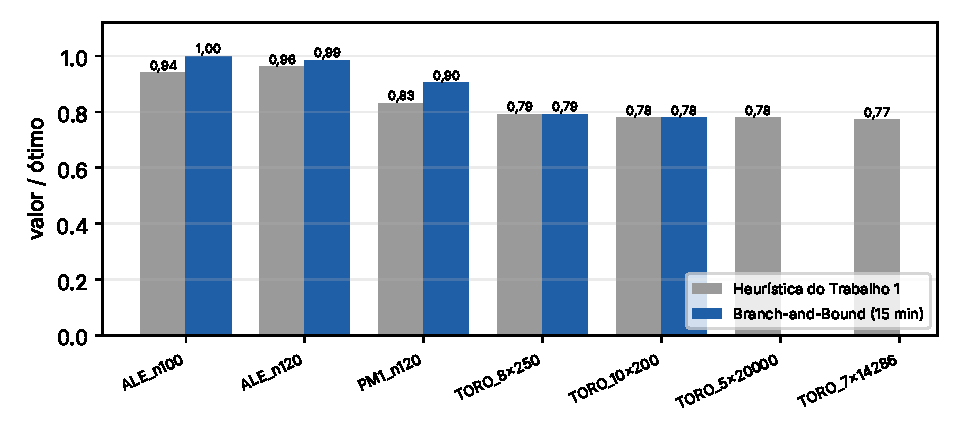
\includegraphics[width=0.92\textwidth]{fig_razao.pdf}
\caption{Valor obtido em relação ao ótimo nas instâncias em que a programação dinâmica calculou o ótimo: heurística do Trabalho~1 (cinza) e Branch-and-Bound com 15 minutos (azul). O Branch-and-Bound não roda nas instâncias de 100 mil vértices.}\label{fig:razao}
\end{figure}

\begin{figure}[ht]
\centering
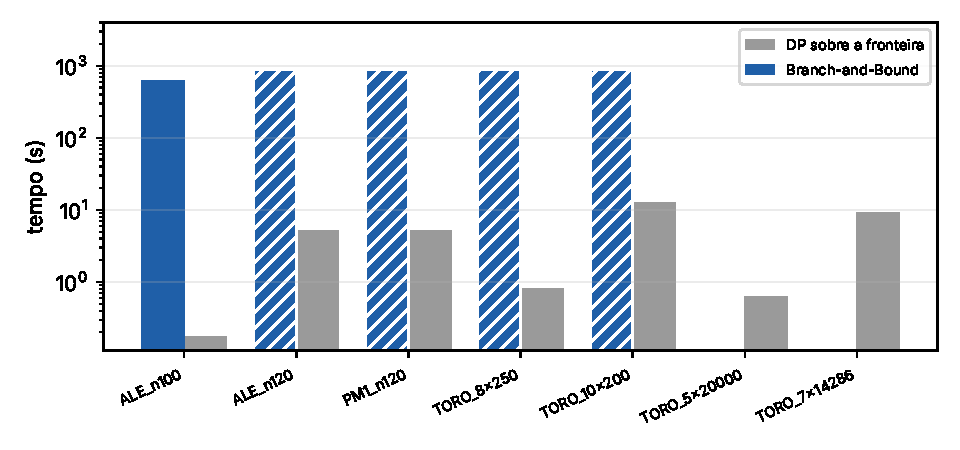
\includegraphics[width=0.92\textwidth]{fig_tempos.pdf}
\caption{Tempo do Branch-and-Bound (azul) e da programação dinâmica (cinza), em escala logarítmica. Barras hachuradas: o Branch-and-Bound parou no limite de 900\,s sem provar o ótimo.}\label{fig:tempos}
\end{figure}

\subsection{Programação dinâmica}

A programação dinâmica calculou o ótimo das 7 instâncias dos grupos A e B, inclusive as duas grades de cerca de 100 mil vértices, em 0,63\,s ($w=11$) e 9,2\,s ($w=15$). O tempo depende de $w$, e quase nada de $n$: cada 4 unidades a mais de largura multiplicam o tempo por cerca de 16 ($0{,}81$\,s com $w=17$ e $12{,}9$\,s com $w=21$, ambas com 2\,000 vértices), como previsto por $O(2^{w}(n+m))$. A memória acompanha: de 12\,MB ($w=11$) a 845\,MB ($w=26$, o limite da implementação). Nas instâncias do grupo C, a fronteira encontrada é de 41 ou mais, e a programação dinâmica não executa.

\subsection{Branch-and-Bound}

O Branch-and-Bound só provou a otimalidade de uma instância, a \texttt{01\_ALE\_n100} (ótimo 168), em 620\,s e $1{,}9\cdot10^{10}$ nós. A programação dinâmica resolve a mesma instância em 0,17\,s, cerca de 3\,600 vezes mais rápido. Nas outras 9 instâncias ele chegou ao limite de 15 minutos, depois de visitar entre 31 e 52 bilhões de nós. É um número enorme, mas pequeno diante do espaço de busca ($2^{120}$ em $n=120$; $2^{2000}$ no G32).

O motivo é que o teto é folgado. Na coluna ``Limitante inicial'' da Tabela~\ref{tab:bb}, vemos que, antes de decidir qualquer vértice, o teto já está de 18\% a 88\% acima do valor final. Nas instâncias com pesos $+1$ o teto inicial vale exatamente $m$ (200, 240 e 400): ele supõe que todas as arestas podem ser cortadas, enquanto o ótimo corta cerca de 85\% delas. Nas grades, onde metade das arestas tem peso negativo, o teto inicial é 2\,001 contra um ótimo de 1\,406 e 1\,386. Com um teto assim, só se poda quando já se perdeu muito, e isso demora a acontecer.

Mesmo assim, o Branch-and-Bound melhorou a heurística do Trabalho~1 em 5 das 10 instâncias em que roda (Figura~\ref{fig:razao}). Nas aleatórias pequenas ele chegou perto do ótimo: 168 de 168 na \texttt{01} (a heurística tinha 158), 201 de 204 na \texttt{02} (heurística 196) e 75 de 83 na \texttt{03} (heurística 69). Nas grades de 2\,000 vértices (04 e 05) não houve nenhuma melhoria em 15 minutos: o valor final é o da heurística (1\,114 e 1\,080), bem abaixo do ótimo (1\,406 e 1\,386). No grupo C, onde o ótimo é desconhecido, ele melhorou a \texttt{08} (de 316 para 322) e a \texttt{10} (de 516 para 528), e não alterou a \texttt{09}, o G32 e o G57. Como o teto inicial fica de 70\% a 73\% acima desses valores, não dá para saber se a heurística é ótima ou não nessas três: o Branch-and-Bound entrega uma solução, mas nenhuma garantia.

\subsection{Comparação com o Trabalho 1}

Com os ótimos em mãos, dá para medir a heurística do Trabalho~1 contra o valor verdadeiro. Nas grades toroidais ela obtém de 77\% a 79\% do ótimo (0,792; 0,779; 0,778 e 0,772), e a razão não piora com o tamanho: com 100 mil vértices é praticamente a mesma que com 2\,000. Nas aleatórias esparsas com pesos $+1$ ela obtém 0,94 e 0,96 (na faixa de 93\% a 96\% relatada no Trabalho~1) e, com pesos $\pm1$, 0,83. Esses valores são da mesma ordem dos 80\% a 82\% do melhor valor conhecido que o Trabalho~1 relatou nos toroidais do G-set, o que sugere que a diferença se deve sobretudo à busca local, e não a uma referência frouxa. Para o G32 e o G57 não podemos afirmar o mesmo: a versão da heurística incorporada ao programa novo dá 1\,170 e 2\,924 (0,83 e 0,84 dos melhores valores conhecidos, 1\,410 e 3\,494), um pouco acima dos 0,82 do relatório anterior. Ou seja, o desempate da ordenação por grau já move o resultado em 1\% a 3\%. O Branch-and-Bound não alterou esses dois valores.

O preço do ótimo também fica claro: a heurística leva de 8\,$\mu$s (100 vértices) a 12\,ms (100 mil vértices); a programação dinâmica, de 0,17\,s a 13\,s onde roda; e o Branch-and-Bound, 10 minutos para provar uma instância de 100 vértices e mais de 15 minutos nas demais. A heurística é a melhor escolha quando o tempo importa; os algoritmos exatos servem para medir quanto ela deixa de ganhar, que nas grades é de 21\% a 23\% do ótimo.

\subsection{Comparação com a literatura}

Não dá para comparar tempos diretamente com os resolvedores da literatura: não usamos as instâncias da \emph{Biq Mac Library} nem os códigos do \emph{Biq Mac} e do \emph{BiqCrunch}, e as máquinas são diferentes. O que podemos dizer é qualitativo. O \emph{Biq Mac} resolve qualquer instância de até 100 vértices, mesmo densa \cite{Rendl et al. 2010}; nosso Branch-and-Bound provou uma instância esparsa de 100 vértices em 10 minutos e não resolveu as de 120, o que é esperado, pois seu teto é bem mais fraco que o semidefinido. A programação dinâmica resolve aleatórios esparsos até 120 vértices em 5\,s, mas só porque são esparsos; em grafos densos seria inviável. O branch-and-cut de \citet{Liers et al. 2003} chega a 1\,280 vértices em grafos aleatórios de grau 4, uma ordem de grandeza acima do que alcançamos (a \texttt{08\_ALE\_n200} está fora do alcance da nossa programação dinâmica). Nossas grades de 100 mil vértices só são resolvidas porque a largura é pequena, e não porque o algoritmo seja mais forte.

\subsection{Limitações}

Cada instância foi executada uma vez, em uma única máquina, e há uma instância por tipo e tamanho, então os resultados mostram o comportamento, mas não são uma estatística. O limite de 900\,s é arbitrário; com mais tempo o Branch-and-Bound poderia provar alguma instância pequena a mais. A ordem da programação dinâmica é heurística, e uma ordem melhor poderia resolver instâncias maiores (nas do grupo C só estimamos a largura com poucas tentativas). Nas instâncias 08 a 12 o ótimo é desconhecido, e o valor final do Branch-and-Bound é só um limite inferior para ele.

\section{Conclusão}

Implementamos e validamos dois algoritmos exatos para o Corte Máximo, um Branch-and-Bound e uma programação dinâmica sobre a fronteira, ambos com prova de correção e análise de custo. Em 12 instâncias de 100 a 100\,002 vértices, com limite de 15 minutos por algoritmo, a programação dinâmica calculou o ótimo de 7, inclusive duas grades toroidais de cerca de 100 mil vértices (em 0,63\,s e 9,2\,s), porque a fronteira é pequena. O Branch-and-Bound provou a otimalidade de uma instância (100 vértices, 620\,s) e esgotou o tempo nas demais, porque seu teto é folgado; mesmo assim, devolveu soluções melhores que as da heurística em 5 das 10 instâncias em que roda.

Com os ótimos, confirmamos o diagnóstico do Trabalho~1: a heurística gulosa com busca local obtém de 77\% a 79\% do ótimo nas grades toroidais com pesos $\pm1$, de 2\,000 a 100 mil vértices, e de 83\% a 96\% em aleatórias esparsas pequenas. As instâncias do G-set (G32 e G57) continuam fora do alcance dos dois algoritmos.

Como trabalho futuro, o ganho mais claro está em tetos melhores para o Branch-and-Bound (por exemplo, com programação linear ou semidefinida, como a literatura faz) e em ordens melhores para a programação dinâmica. Também valeria rodar os algoritmos nas instâncias da \emph{Biq Mac Library}, para uma comparação direta com a literatura.

\renewcommand{\refname}{Referências}
\begin{thebibliography}{99}
\small
\bibitem[Arnborg et al.(1991)]{Arnborg et al. 1991} Arnborg, S., Lagergren, J., and Seese, D. (1991). Easy problems for tree-decomposable graphs. \emph{Journal of Algorithms}, 12(2).

\bibitem[Barahona et al.(1988)]{Barahona et al. 1988} Barahona, F., Grötschel, M., Jünger, M., and Reinelt, G. (1988). An application of combinatorial optimization to statistical physics and circuit layout design. \emph{Operations Research}, 36(3).

\bibitem[Benlic and Hao(2013)]{Benlic and Hao 2013} Benlic, U. and Hao, J.-K. (2013). Breakout local search for the Max-Cut problem. \emph{Engineering Applications of Artificial Intelligence}, 26(3).

\bibitem[Bodlaender(1993)]{Bodlaender 1993} Bodlaender, H. L. (1993). A tourist guide through treewidth. \emph{Acta Cybernetica}, 11(1--2).

\bibitem[Garey et al.(1976)]{Garey et al. 1976} Garey, M. R., Johnson, D. S., and Stockmeyer, L. (1976). Some simplified NP-complete graph problems. \emph{Theoretical Computer Science}, 1(3).

\bibitem[Hadlock(1975)]{Hadlock 1975} Hadlock, F. (1975). Finding a maximum cut of a planar graph in polynomial time. \emph{SIAM Journal on Computing}, 4(3).

\bibitem[Karp(1972)]{Karp 1972} Karp, R. M. (1972). Reducibility among combinatorial problems. In \emph{Complexity of Computer Computations}. Plenum Press.

\bibitem[Kinnersley(1992)]{Kinnersley 1992} Kinnersley, N. G. (1992). The vertex separation number of a graph equals its path-width. \emph{Information Processing Letters}, 42(6).

\bibitem[Krislock et al.(2014)]{Krislock et al. 2014} Krislock, N., Malick, J., and Roupin, F. (2014). Improved semidefinite bounding procedure for solving Max-Cut problems to optimality. \emph{Mathematical Programming}, 143(1--2).

\bibitem[Liers et al.(2003)]{Liers et al. 2003} Liers, F., Palassini, M., Hartmann, A. K., and Jünger, M. (2003). Ground state of the Bethe lattice spin glass and running time of an exact optimization algorithm. \emph{Physical Review B}, 68(9).

\bibitem[Liers et al.(2004)]{Liers et al. 2004} Liers, F., Jünger, M., Reinelt, G., and Rinaldi, G. (2004). Computing exact ground states of hard Ising spin glass problems by branch-and-cut. In Hartmann, A. K. and Rieger, H., editors, \emph{New Optimization Algorithms in Physics}. Wiley-VCH.

\bibitem[Rendl et al.(2010)]{Rendl et al. 2010} Rendl, F., Rinaldi, G., and Wiegele, A. (2010). Solving Max-Cut to optimality by intersecting semidefinite and polyhedral relaxations. \emph{Mathematical Programming}, 121(2).

\bibitem[Williams(2005)]{Williams 2005} Williams, R. (2005). A new algorithm for optimal 2-constraint satisfaction and its implications. \emph{Theoretical Computer Science}, 348(2--3).
\end{thebibliography}

\end{document}
